% \begin{theorem}
%     Suppose that \textbf{either} of the two statements hold for some $\mcl{V}$ or corresponding dual $\mcl{V}'$ and $\mcl{P}\in\Pi_4$ such that $\mcl{P}=\mcl{P}^*\succeq 0$
%     \begin{enumerate}
%         \item \begin{equation*}
%         \bmat{\mcl{A}^*\mcl{P}\mcl{T} + \mcl{T}^*\mcl{P}\mcl{A} & \mcl{T}^*\mcl{P}\mcl{B} +\mcl{C}^*\mcl{V}_{12} & \mcl{C}^*\mcl{V}^*_{11}\\\mcl{B}^*\mcl{P}\mcl{T}+\mcl{V}_{21}\mcl{C} & \mcl{V}_{21}\mcl{D}+\mcl{D}^*\mcl{V}_{12} + \mcl{V}_{22} & \mcl{D}^*\mcl{V}^*_{11} \\ \mcl{V}_{11}\mcl{C} & \mcl{V}_{11}\mcl{D} & -\mcl{V}_{11}} \preceq 0
%         \end{equation*}
%         \item \begin{equation*}
%         \bmat{\mcl{A}\mcl{P}\mcl{T}^* + \mcl{T}\mcl{P}\mcl{A}^* & \mcl{T}\mcl{P}\mcl{C}^* +\mcl{B}\mcl{V}'_{12} & \mcl{B}{\mcl{V}'}^{*}_{11}\\\mcl{C}\mcl{P}\mcl{T}^*+\mcl{V}'_{21}\mcl{B}^* & \mcl{V}'_{21}\mcl{D}^*+\mcl{D}\mcl{V}'_{12} + \mcl{V}'_{22} & \mcl{D}{\mcl{V}'}^*_{11} \\ \mcl{V}'_{11}\mcl{B}^* & \mcl{V}'_{11}\mcl{D}^* & -\mcl{V}'_{11}} \preceq 0
%         \end{equation*}
%     \end{enumerate}
%     Then, for any $w(t)\in\RL^{\mbf{n}_w}$ and $z(t)$ that satisfies
%     \begin{equation*} 
%     \bmat{\partial_t(\mcl{T}\mbf{x}_f(t)) \\ z(t)} = \bmat{\mcl{A} & \mcl{B} \\ \mcl{C} & \mcl{D}}\bmat{\mbf{x}_f(t) \\ w(t)}
%     \end{equation*}
% \end{theorem}


As a practical first
step, it is generally advisable to synthesize a controller for the nominal
system before accounting for uncertainties. In addition, we incorporate
performance specifications through weighting filters. This is a standard
technique in optimal and robust control synthesis for finite dimensional
systems by embedding frequency-dependent performance characteristics into the
synthesis.

\begin{figure}[h]
	\centering
	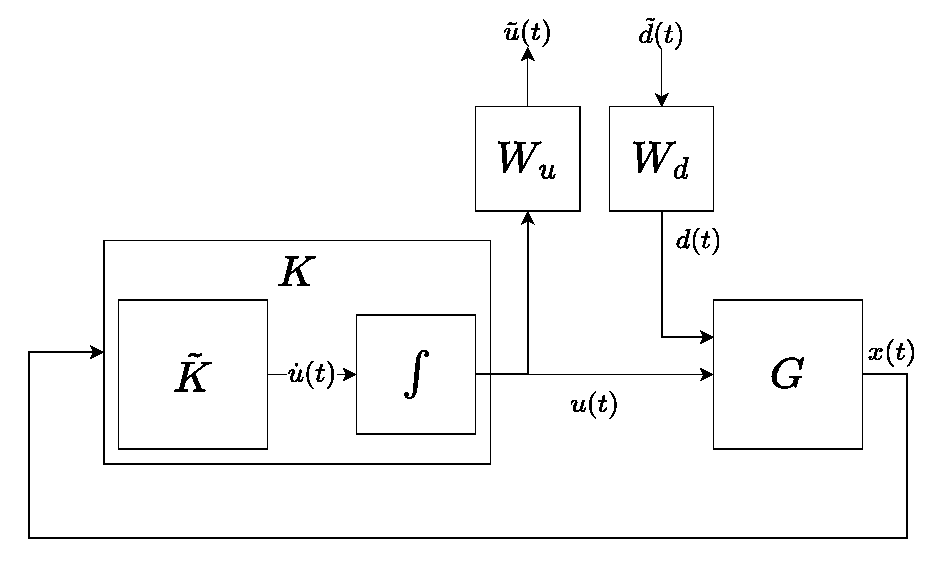
\includegraphics[width=1\linewidth]{Figures/Filtered_Optimal_Control.eps}
	\caption{
		Block schematic of the weighted diffusion--reaction system with boundary
		control, where $W_u$ characterizes the inverse frequency-dependent
		characteristics of the desired control input $u(t),$ and $W_d$
		characterizes the frequency content of the disturbance, i.e.,
		$\tilde{u}(t) = W_u u(t)$ and $w(t) = W_d \tilde{w}(t)$.
	}
	\label{fig:weightedsystem}
\end{figure}
\begin{figure}[h]
	\centering
	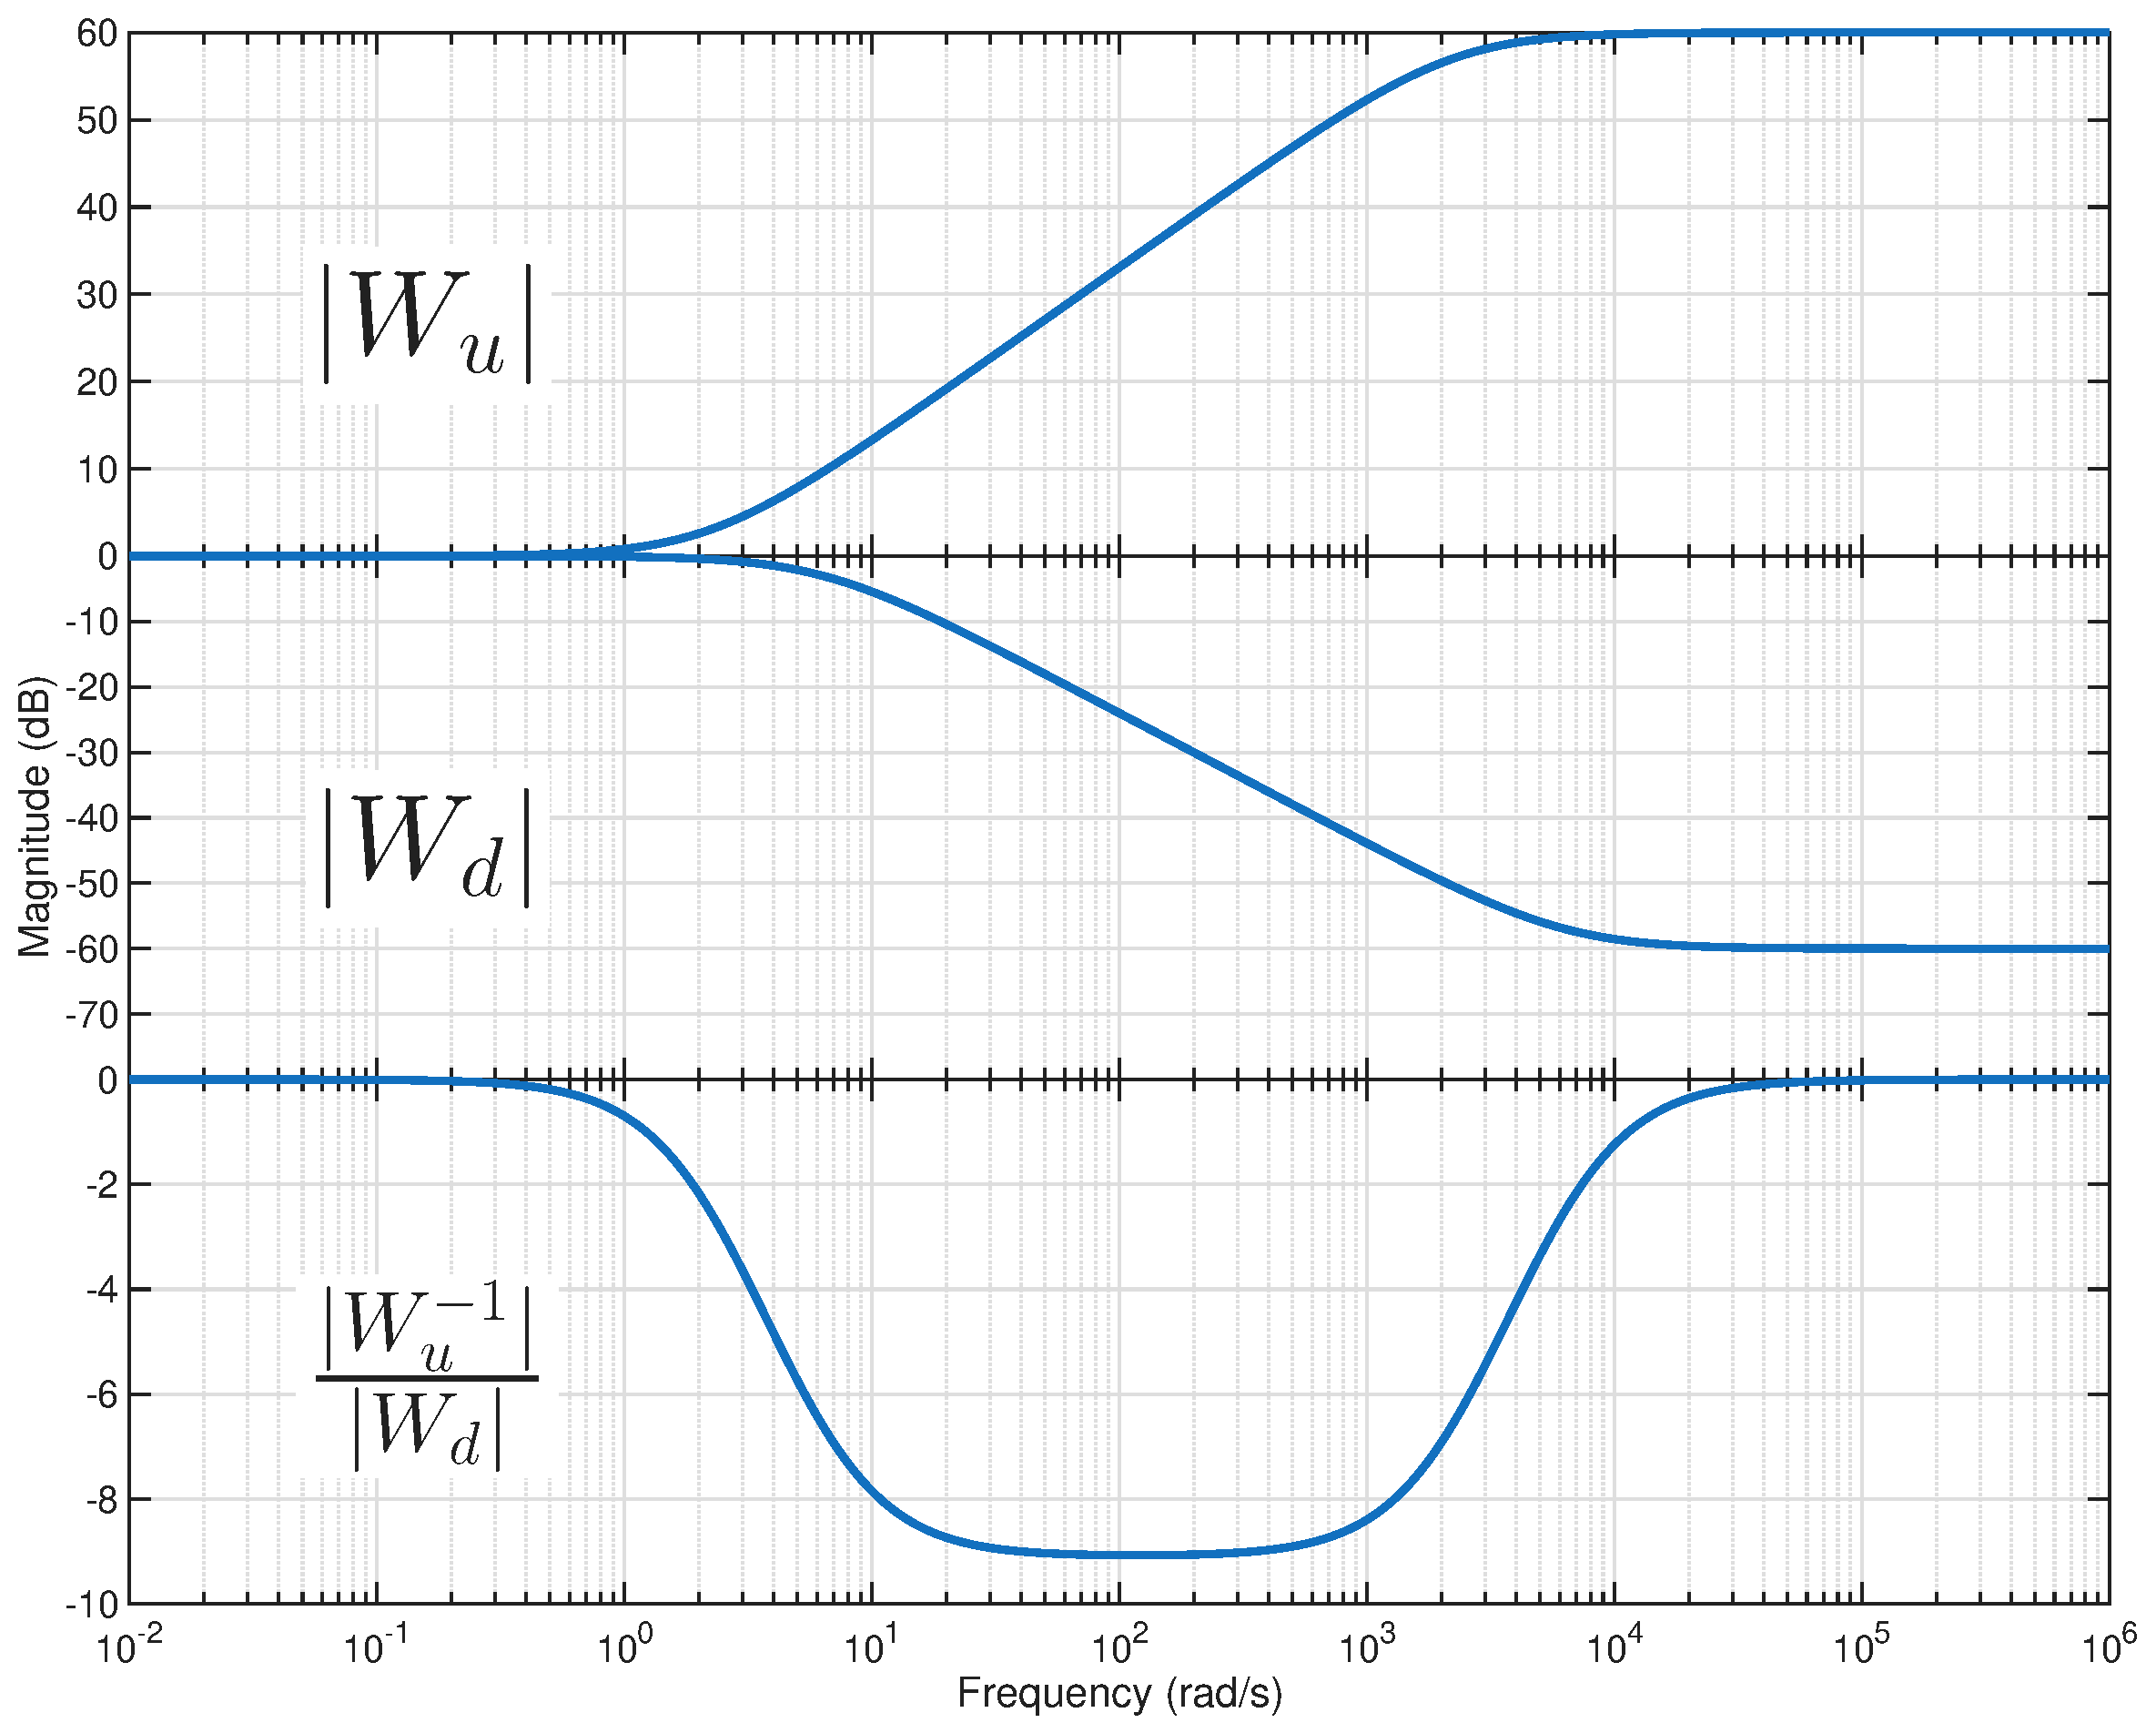
\includegraphics[width=1\linewidth]{Figures/weighting_filters.eps}
	\caption{
		Bode magnitude plots of the input and disturbance weighting filters,
		$W_u$ and $W_d$, together with the combined inverse weighting
		$W_u^{-1}W_d^{-1}$. These weights are used to encode the desired
		frequency-dependent characteristics of the control input and disturbance
		in the weighted boundary control synthesis.
	}
	\label{fig:freqchar}
\end{figure}
\noindent We begin by considering the boundary control problem for a
diffusion--reaction equation, adapted from \cite{shivaknew}. Throughout, we
assume that the disturbance and control input are measurable, as the
introduction of weighting filters gives rise to additional states that depend
explicitly on these signals.
\begin{example}[Reaction--Diffusion Equation]
	Consider the boundary control of an unstable reaction--diffusion equation:
	\begin{equation*}
		\begin{aligned}
			\dot{\mbf{v}}(t,s)     & = 5\mbf{v}(t,s) + \partial_s^2 \mbf{v}(t,s) + C_{\tilde{d}}x_{\tilde{d}}(t) + D_{\tilde{d}}\tilde{d}(t), \\
			\dot{x}_{u}(t)         & = \dot{u}(t),                                                                                            \\
			\dot{x}_{\tilde{u}}(t) & = A_{\tilde{u}}x_{\tilde{u}}(t) + B_{\tilde{u}}x_u(t),                                                   \\
			\dot{x}_{\tilde{d}}(t) & = A_{\tilde{d}}x_{\tilde{d}}(t) + B_{\tilde{d}}\tilde{d}(t),                                             \\
			z(t)                   & = \tilde{u}(t) = C_{\tilde{u}}x_{\tilde{u}}(t) + D_{\tilde{u}}x_u(t),                                    \\
			\mbf{v}(t,0)           & = 0, \qquad \partial_s \mbf{v}(t,1) = x_u(t).
		\end{aligned}
	\end{equation*}
	Here, the state $x_{\tilde{u}}$ embeds the frequency characteristics of the
	weighting filter $W_u$, while $x_{\tilde{d}}$ embeds those of the weighting
	filter $W_d$ shown in Fig.~\ref{fig:freqchar}. Moreover, the input $u$ is
	passed through an integrator so that the control input does not act directly
	on the boundary. This ensures that $\mathcal{T}_u = 0$, which is required
	for synthesis. Solving the associated synthesis conditions yields an
	$\mathcal{H}_\infty$ gain of $\gamma = 0.9773$, that is,
	\[
		\frac{\|\tilde{u}\|_{L_2}}{\|\tilde{d}\|_{L_2}} < 0.9773.
	\]
	This performance is achieved together with an exponential decay rate of $\alpha = 2$.
\end{example}
\DeclareRobustCommand{\estimatedtransferlegend}{%
	\tikz[baseline=-0.6ex]\draw[blue,line width=0.8pt] (0,0) -- (0.4,0);%
}
\DeclareRobustCommand{\targetprofilelegend}{%
	\tikz[baseline=-0.6ex]\draw[orange,line width=0.8pt,dashed] (0,0) -- (0.4,0);%
}
\begin{figure}[h]
	\centering
	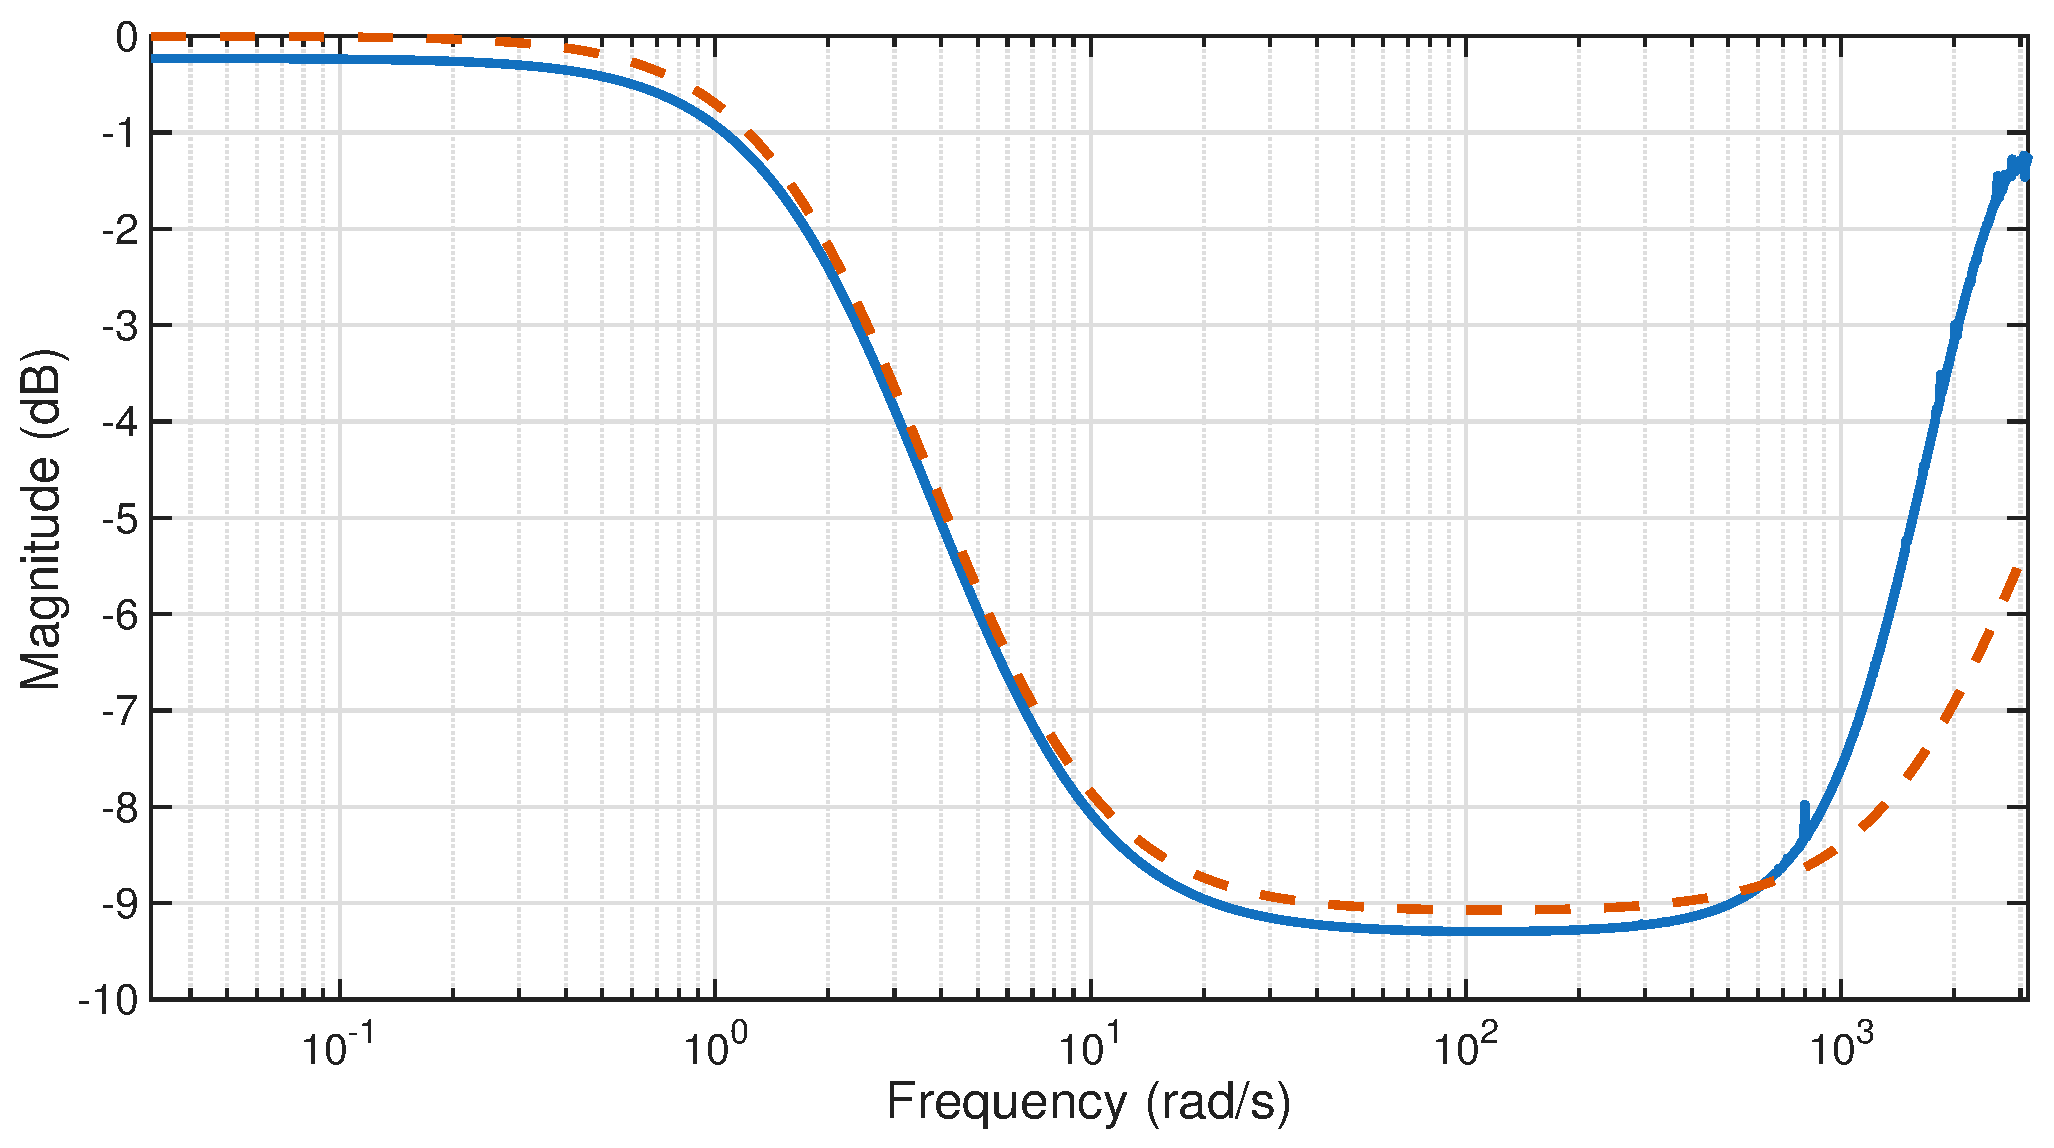
\includegraphics[width=1\linewidth]{Figures/emperical_estimate.eps}
	\caption[Empirical frequency-response estimate from disturbance input to control input.]{
		Empirical frequency-response estimate from the disturbance input to the
		control input over the range $0.1$ rad/s to $10^4$ rad/s.
		\estimatedtransferlegend\ $\frac{|U|}{|W|}$ denotes the estimated
		transfer magnitude, while \targetprofilelegend\
		$\frac{|W_u^{-1}|}{|W_d|}$ denotes the target weighting profile.
	}
	\label{fig:empiricalestimate}
\end{figure}
To assess whether the weighting specifications are met in practice, we compute
an empirical transfer function estimate from the disturbance channel to the
control input. For this purpose, we excite the system with a unit-amplitude
frequency sweep ranging from $0.1$ rad/s to $10^{4}$ rad/s, filtered through
the disturbance weighting filter $W_d$. The resulting signal is applied as the
disturbance input, while the corresponding control input is measured. An
estimate of the associated frequency response is then obtained from the Fourier
transforms of these signals. Comparing this estimate with the desired weighted
behavior allows us to verify that the imposed frequency-domain design
specifications are achieved.
